\subsubsection{Architektur des Generators}
Die Architektur der Generatoren in CycleGAN spielt eine entscheidende Rolle bei der erfolgreichen Durchführung von Bildübersetzungen zwischen verschiedenen Domänen. Typischerweise basieren die Generatoren auf dem ResNet-Ansatz, der für seine Fähigkeit bekannt ist, tiefe neuronale Netze zu trainieren\cite{He.2015}.
\\

\begin{figure}[ht]
	\centering
	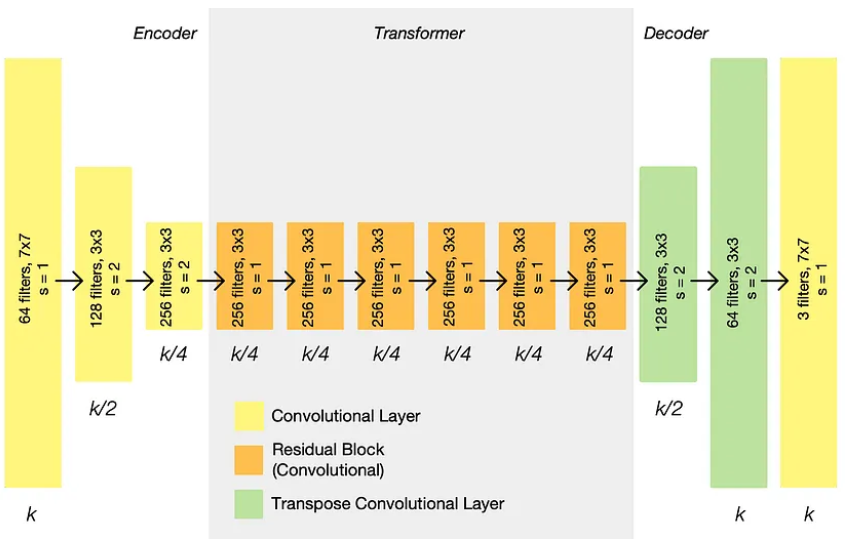
\includegraphics[width=0.8\linewidth]{./images/cycleGanGeneratorArchitecture.png}
	\caption{Eine Architektur eines CycleGAN Generator. Instanznormalisierung und ReLU Aktivierung erfolgt nach jeder Schicht
	\protect\footnotemark}
	\label{fig:cycleGanGeneratorArchitecture}
\end{figure}
\footnote[1]{https://towardsdatascience.com/cyclegan-learning-to-translate-images-without-paired-training-data-5b4e93862c8d}

Im Rahmen der Architektur von Zhu et al. manifestiert sich der Generator im CycleGAN in drei zentralen Abschnitten, wie graphisch in Abbildung \ref{fig:cycleGanGeneratorArchitecture} illustriert. Der Encoder besteht aus drei Convolutional-Schichten, welche unmittelbar auf das Eingabebild einwirken und dabei die Repräsentationsgröße reduzieren, sowie die Kanalanzahl erhöhen. Das resultierende Bild unterzieht sich einem Transformer, zusammengesetzt aus mehreren Residualblöcken. Die aus dieser Transformation hervorgehende Repräsentation durchläuft den Decoder, welcher aus zwei Transpose-Convolutional-Schichten besteht und somit das Bild erneut vergrößert. Die finale RGB-Ausgabe wird durch eine Ausgabeschicht generiert. Jede dieser Schichten ist mit einer Instanznormalisierung und ReLU-Aktivierung versehen, was sowohl die Trainingsstabilität fördert, als auch die Qualität der generierten Bilder optimiert\cite{Ulyanov.2016,Nair.2010}. 
\\
\newline
Die ResNet-Methode, von Kaiming He et al. im Jahr 2015 eingeführt, bietet eine Lösung für das Degradationsproblem. Dieses Phänomen tritt auf, wenn tiefe neuronale Netze bei Zugabe zusätzlicher Schichten schlechtere Leistungen erbringen als flachere Netze, da die Rückwärtspropagierung von Fehlern in tieferen Netzwerken erschwert wird. Die Integration von Residualblöcken ermöglicht die Überwindung dieses Problems durch die Hinzufügung einer Identitätsabbildung. Das Netzwerk lernt diese Abbildung, indem es das Residuum auf Null setzt. Residualblöcke dienen dazu, Änderungen und Fehler zu erlernen, die notwendig sind, um von der Eingabe zur gewünschten Ausgabe zu gelangen. Dies wird durch Shortcut-Verbindungen realisiert, die eine oder mehrere Ebenen überspringen und am Ende einer gestapelten Schicht hinzugefügt werden. Solche Verbindungen fügen keine zusätzlichen Parameter oder Rechenleistung hinzu, und das gesamte Netzwerk kann weiterhin mittels stochastischem Gradientenabstieg (SDG) trainiert werden\cite{He.2015}.

\begin{figure}[ht]
	\centering
	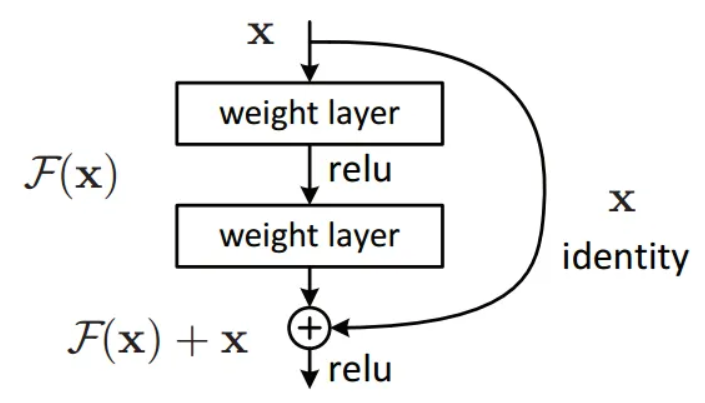
\includegraphics[width=0.5\linewidth]{./images/residualBlock.png}
	\caption{Ein Aufbau eines Residualblocks}
	\label{fig:residualBlock}
\end{figure}

\subsubsection{Architektur des Diskriminators}
In Pix2Pix ist die gängige Architektur für Diskriminatoren ein PatchGAN, bei dem das Bild in kleine Patches unterteilt wird und jeder Patch separat klassifiziert wird (vgl. Abschnitt \ref{sec:PatchGAN}). Diese Vorgehensweise ermöglicht eine präzise Unterscheidung zwischen echten und generierten Bildern auf lokaler Ebene, was besonders in Bezug auf die feinstrukturierte Bewertung von Bildabschnitten von Vorteil ist \cite{Zhu.2017}.
\newline
In den Implementierungen von CycleGAN wird im Unterschied zu Pix2Pix auf die Verwendung von Batch-Normalisierung verzichtet, und stattdessen wird Instanznormalisierung bevorzugt. Bei der Instanznormalisierung wird jedes Bild individuell betrachtet, ohne Berücksichtigung über die gesamte Batch-Dimension hinweg. Dieser Ansatz bietet eine effektivere Stilübertragung im Feed-Forward-Modus und weist eine schnellere Konvergenz auf im Vergleich zur Batch Normalisierung \cite{Huang.2017}. Eine mögliche Architektur ist in Abbildung \ref{fig:PatchGANDiskriminator} veranschaulicht.

\subsubsection{Training}
Das Training von CycleGAN erfolgt nach einem kompetitiven Verfahren. Die Generatoren $G:X\rightarrow Y$ und $F:Y\rightarrow X$ konkurrieren mit den entsprechenden Diskriminatoren $D_X$ und $D_Y$. $D_X$ versucht, die von $F$ erzeugten Bilder von den echten Bildern aus $X$ zu unterscheiden, während $D_Y$ versucht, die von $G$ erzeugten Bilder von den echten Bildern aus der Domäne $Y$ zu unterscheiden \ref{fig:cycleConsistency}. Die adversen Verluste sind so optimiert, dass die erzeugten Bilder für die Diskriminatoren kaum von den echten Bildern zu unterscheiden sind. \cite{Zhu.2017}.

\subsubsection{Cycle - Konsistenz}
CycleGAN führt zusätzlich eine Cycle-Konsistenz ein. Diese stellt sicher, dass die Übersetzungen zwischen den Domänen sowohl vorwärts ($X$ nach $Y$), als auch rückwärts ($Y$ nach $X$) konsistent sind. Dies ist in der Abbildung \ref{fig:cycleConsistency} dargestellt.
\\
Die Kernidee besteht darin, dass nach der Übersetzung von $X$ nach $Y$ und zurück nach $X$ das resultierende Bild dem ursprünglichen $X$ entsprechen sollte. Um dies zu erreichen, wird die Differenz zwischen dem Originalbild $x$ und dem zyklisch übersetzten Bild $F(G(x))$ mit Hilfe der L1-Verlust minimiert. 
\\
Durch die Einführung dieser zyklischen Konsistenz stellt ein Ansatz zur Lösung des Problem des Modekollapses dar. Die weitere Verlustfunktion stellt sicher, dass die generierten Bilder mehr Strukturen enthalten und somit konsistentere Übersetzungen zwischen den Domänen liefern \cite{Zhu.2017}.

\begin{figure}[ht]
	\centering
	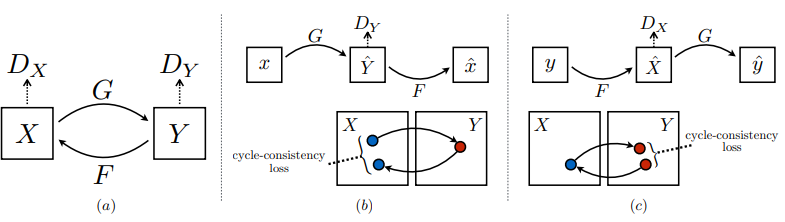
\includegraphics[width=1\linewidth]{./images/cycle_consistency_loss.png}
	\caption{(a) Modell des CycleGANs, bestehend aus zwei Generatoren $F:Y\rightarrow X$ und $G:X \rightarrow Y$ und zugehörige adversarielle Diskriminatoren $D_X$ und $D_Y$,
     (b) Cycle-Konsistenz $F(G(x))\approx x$,
     (c) Cycle-Konsistenz $G(F(y))\approx y$\cite{Zhu.2017}}
	\label{fig:cycleConsistency}
\end{figure}

\subsubsection{Identity - Loss}
Zusätzlich zu den adversariellen und zyklischen Verlusten kann ein Identitätsverlust in die Gesamtverlustfunktion integriert werden, um sicherzustellen, dass die Farbkomposition des Eingabebildes beibehalten wird, während es ins Ausgabebild übersetzt wird. Insbesondere bei der Erstellung von Fotografien aus Gemälden hat sich diese Methode bewährt.  
Wenn der Generator $G$ ein Bild aus dem Bereich $Y$ erhält, darf es sich aufgrund seiner bereits vorhandenen Zugehörigkeit zu diesem Bereich nicht mehr verändern. Diese Unveränderlichkeit ist visuell veranschaulicht in Abbildung \ref{fig:IdentityMapping}.
Der Verlust wird dabei mittels des L1-Verlust ermittelt, bei dem die Differenz zwischen den Pixeln des generierten Bildes $G(y)$ und dem Referenzbild $y\in Y$ erfasst wird. Das gleiche Verfahren wird für den anderen Generator $F$ angewendet \cite{Zhu.2017}

\begin{figure}[h]
	\centering
	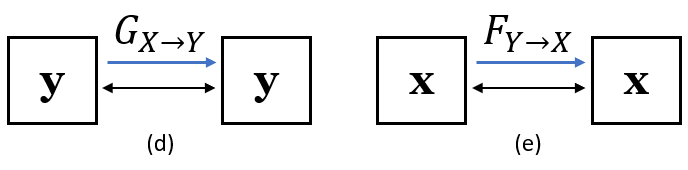
\includegraphics[width=0.7\linewidth]{./images/identity_loss.png}
	\caption{Identity-Mapping für (d) Generator $G$ und (e) Generator $F$}
	\label{fig:IdentityMapping}
\end{figure}


\subsection{Anwendungen von CycleGAN}
CycleGAN hat sich als äußerst vielseitiges Modell erwiesen und findet Anwendung in einer Vielzahl von Bereichen. Insbesondere seine Fähigkeit zur Bildübersetzung zwischen unpaaren Domänen hat zu zahlreichen innovativen Anwendungen geführt. Eine herausragende Nutzung von CycleGAN liegt in der Bild-zu-Bild-Übersetzung und Stilübertragung. Durch dieses Modell können Bilder zwischen verschiedenen Stilen, Szenarien oder Kunstwerken transformiert werden, wodurch die Generierung verschiedener visueller Ästhetiken in einem Bild ermöglicht wird. Diese Anwendung eröffnet kreative Ansätze in der Bildbearbeitung, wie beispielsweise die Umwandlung von Fotografien in den Stil bekannter Kunstwerke \cite{Zhu.2017}.

Ein weiterer bedeutender Anwendungsbereich von CycleGAN ist die Gesichtsalterung, die in der Gesichtserkennung mit Altersprogression sowie in forensischen Untersuchungen Anwendung finden kann. Die Fähigkeit des Modells, realistische Altersprogressionen in Gesichtsbildern zu erzeugen, stellt einen innovativen Beitrag zu forensischen Methoden dar \cite{Sharma.2022}.

In der Stenografie eröffnet CycleGAN ebenfalls interessante Anwendungsmöglichkeiten. Hier kann es genutzt werden, um Satellitenbilder in Karten von Google Maps umzuwandeln und umgekehrt. Diese Anwendung zeigt die Anpassungsfähigkeit des Modells im Umgang mit unterschiedlichen Datenmodalitäten \cite{Chu.2017}.

Darüber hinaus spielt CycleGAN eine bedeutende Rolle in der medizinischen Bildverarbeitung, indem es die Möglichkeit bietet, Bilder von einer Bildgebungsmodalität in eine andere zu übersetzen, um die Diagnose zu verbessern. Bemerkenswerte Erfolge wurden bereits in der Synthese von MRT-Bildern des Beckenbereichs zu CT-Bildern erzielt \cite{Liu.2021}.

Die Flexibilität und Vielseitigkeit von CycleGAN machen es zu einem bedeutenden Werkzeug in der Bildverarbeitung, das innovative Möglichkeiten in verschiedenen Branchen eröffnet. Die fortlaufende Erforschung und Anwendung dieses Modells versprechen weiterhin bedeutende Fortschritte in der digitalen Bildtransformation und -interpretation.